\documentclass[a4paper, 10pt]{article}

\usepackage[margin = 1in]{geometry} % for spacing around
\usepackage{graphicx} % for including images in your pdfs
\usepackage{xcolor} % for including colors in your pdf
\usepackage{soul} % for text decoration
\usepackage[utf8]{inputenc} % for encoded text
\usepackage[T1]{fontenc}
\usepackage{setspace} % for setting different line spacings between paragrafs.
\usepackage{enumerate} % for letting us get more detailed enumerate lists
\usepackage{multirow} % to let us combine more rows together
\usepackage{colortbl} % for decorating tables
\usepackage{amsmath} % used for representing more complicated math displays
\usepackage{supertabular}
\usepackage{longtable} % both of these packages are used to making really big tables
\usepackage{wrapfig} % allows us to wrap text around figures
\usepackage{fancyhdr} % for making fancy headers
%\usepackage{bibtex} % for making better bibliographies
\usepackage[pdftex]{hyperref} % for letting us make links
\usepackage{lscape} % Allows us to flip from portrait to landspace
\usepackage{tikz} % for high detailed drawing
\usepackage{multicol} % To put things side by side
\usepackage{rotating} % For rotating objects
% \usepackage{draftwatermark} % For adding watermarks
\usepackage{MnSymbol} % for using multiple symbols
\usepackage{mathtools} % Used for more math symbols
\usepackage{xfrac} % For more complciated fractions and to add derivitives
\usepackage{hyperref} % for hyper links
\usepackage{enumitem} % for better enum lists
\usepackage{tcolorbox} % for adding colored text boxes
\usepackage{bm} % Adding bold text to math inputs
\usepackage{pgfplots} % Used for plotting functions
\usepackage{subcaption} % Used for subfigures

% Setting up the default image path
\graphicspath{{../../global-assets/images/}}

% Implementing authro details
\title{Lab Report number I - Title of the lab report\\
	ENS203 - Electrical Circuits I}
\author{Emre Arapcic-Uevak\\220302289}
\date{}

% Setting up the fancy page style
\fancypagestyle{customStyle}{
	\lhead{} \chead{} \rhead{}
	\lfoot{} \cfoot{\thepage} \rfoot{}
	\renewcommand{\headrulewidth}{0pt}
	\renewcommand{\footrulewidth}{1pt}
}
\pagestyle{customStyle}

% Setting up hyperref options
\hypersetup {
	colorlinks = false,
	citecolor = black,
	filecolor = blue,
	linkcolor = blue,
	urlcolor = blue,
	pdftex
}

% Custom commands
\newcommand{\figref}[1]{Figure~\ref{#1}}


\begin{document}
	\begin{titlepage}
		\begin{center}
			\vspace*{\stretch{1}} % Add vertical space before the title

			{\Large\bfseries Lab Report number 1 \\[0.5em] Resistance and Current Measurement\par}
			\vspace{1cm} % Space between title and course title

			{\large ENS203 – Electrical Circuits I\par}
			\vspace{1cm} % Space between course title and your name/ID

			{\large Emre Arapcic-Uevak \\ 220302289\par}
			\vspace{1cm} % Space between your name/ID and assistant name

			{\large Assistant: Adil Hasanbasic\par}
			\vspace{\stretch{2}} % Variable vertical space between assistant name and bottom
			
\includegraphics[width=0.5\textwidth]{Logo.png}
			\vspace{5mm}
			
			\textsc{\LARGE Internation University of Sarajevo}\\[1.5cm]
			\textsc{\Large ENS203 - Electrical Circuits I}\\[0.5cm]
			
			\rule{\linewidth}{0.5mm} \\[0.4cm]
			{ \huge \bfseries Lab Report number I - Getting on board}\\[0.4cm]
			\rule{\linewidth}{0.5mm} \\[1.5cm]
			
			\vfill
			
			% Bottom of the page
			{\large \today}
		\end{center}
	\end{titlepage}
	\pagebreak

	\tableofcontents
	\pagebreak
	
	\listoffigures
	\pagebreak
	
	\section{Introduction}
		\subsection{Background}
			Get introduced to the laboratory equipment and learn how to measure resistance, voltage and current safely. Learn how to use breadboard to connect components together in series, parallel and mixed configurations. Learn how to use a multimeter to measure resistance, voltage and current.	
		\subsection{Objective}
			\begin{itemize}
				\item Switch in DC power supply, and fix it to 5 V, then measure the 5 V using the multi-meter
				\item When done switch off.
				\item Switch on function generator, and fix it to produce sin wave with 100 Hz, show the signal on a oscilloscope
				\item Switch off
				\item Pick up two unknown resistors, measure them using the multi – meter
				\item Connect them on bread board in series
				\item Connect them on the bread board in parallel
				\item Use more resistors and connect the following circuit on the bread board.
				\begin{figure}[h]
					\centering
					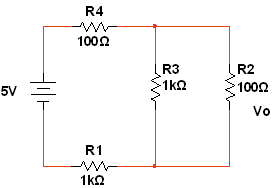
\includegraphics[width=0.5\textwidth]{./images/Task8-Circuit.png}
					\caption{Circuit to be connected on the bread board}
					\label{fig:Task8-Circuit}
				\end{figure}
			\end{itemize}

	\pagebreak
	\section{Methods}
		\subsection{Apparatus}
			\begin{description}
				\item[Breadboard]
					also known as protoboard is a type of solderless electronic circuit board, where you can build electronic circuits without any soldering.
					Its advantages that it is reusable and the circuits are easy to modify and rebuild. \figref{fig:breadboard} shows a part of a breadboard and how the pins are connected,
					although there are many types of breadboards, the principle is the same.

					\begin{figure}[h!]
						\centering
						\begin{subfigure}[h]{0.45\textwidth}
							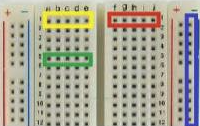
\includegraphics[width=\textwidth]{./images/Breadboard.png}
							\caption{Physical breadboard}
							\label{sub-fig:physical-breadboard}
						\end{subfigure}
						\hspace{0.5cm} % This is the gap between the images
						\begin{subfigure}[h]{0.45\textwidth}
							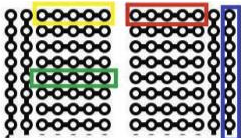
\includegraphics[width=\textwidth]{./images/Breadboard-Connections.png}
							\caption{Breadboard connections}
							\label{sub-fig:breadboard-connections}
						\end{subfigure}

						\caption{Breadboard and its connections}
						\label{fig:breadboard}
					\end{figure}

					Every 5 holes in horizontal direction, which are marked with letters a,b,c,d,e or f,g,h,I,j represent a one connection point.
					When we want to connect circuit elements we connect one terminal of each element in one of the 5 holes, and we connect another element’s terminal into another hole of the 5 to have two elements connected at one point.

					\begin{figure}[h!]
						\centering
						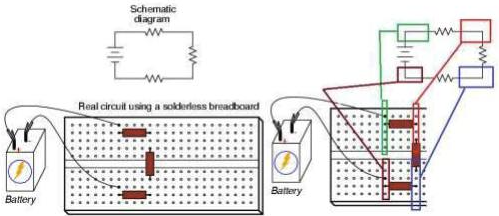
\includegraphics[width=0.7\textwidth]{./images/SchemeDiagramOnABreadboard.png}
						\caption{Scheme diagram on a breadboard}
						\label{fig:SchemeDiagramOnABreadboard}
					\end{figure}

				\item[Multi-meter] used to measure electrical quantities
					\begin{figure}[h!]
						\centering
						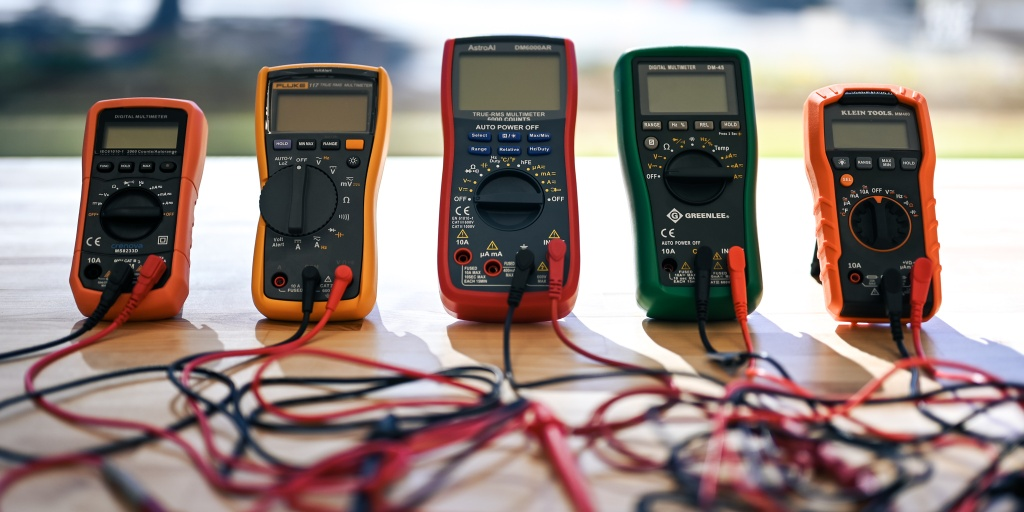
\includegraphics[width=0.5\textwidth]{./images/MultiMeters.jpeg}
						\caption{Multi-meters}
						\label{fig:MultiMeters}
					\end{figure}

				\pagebreak

				\item[DC power supply] used to provide a constant voltage
					\begin{figure}[h!]
						\centering
						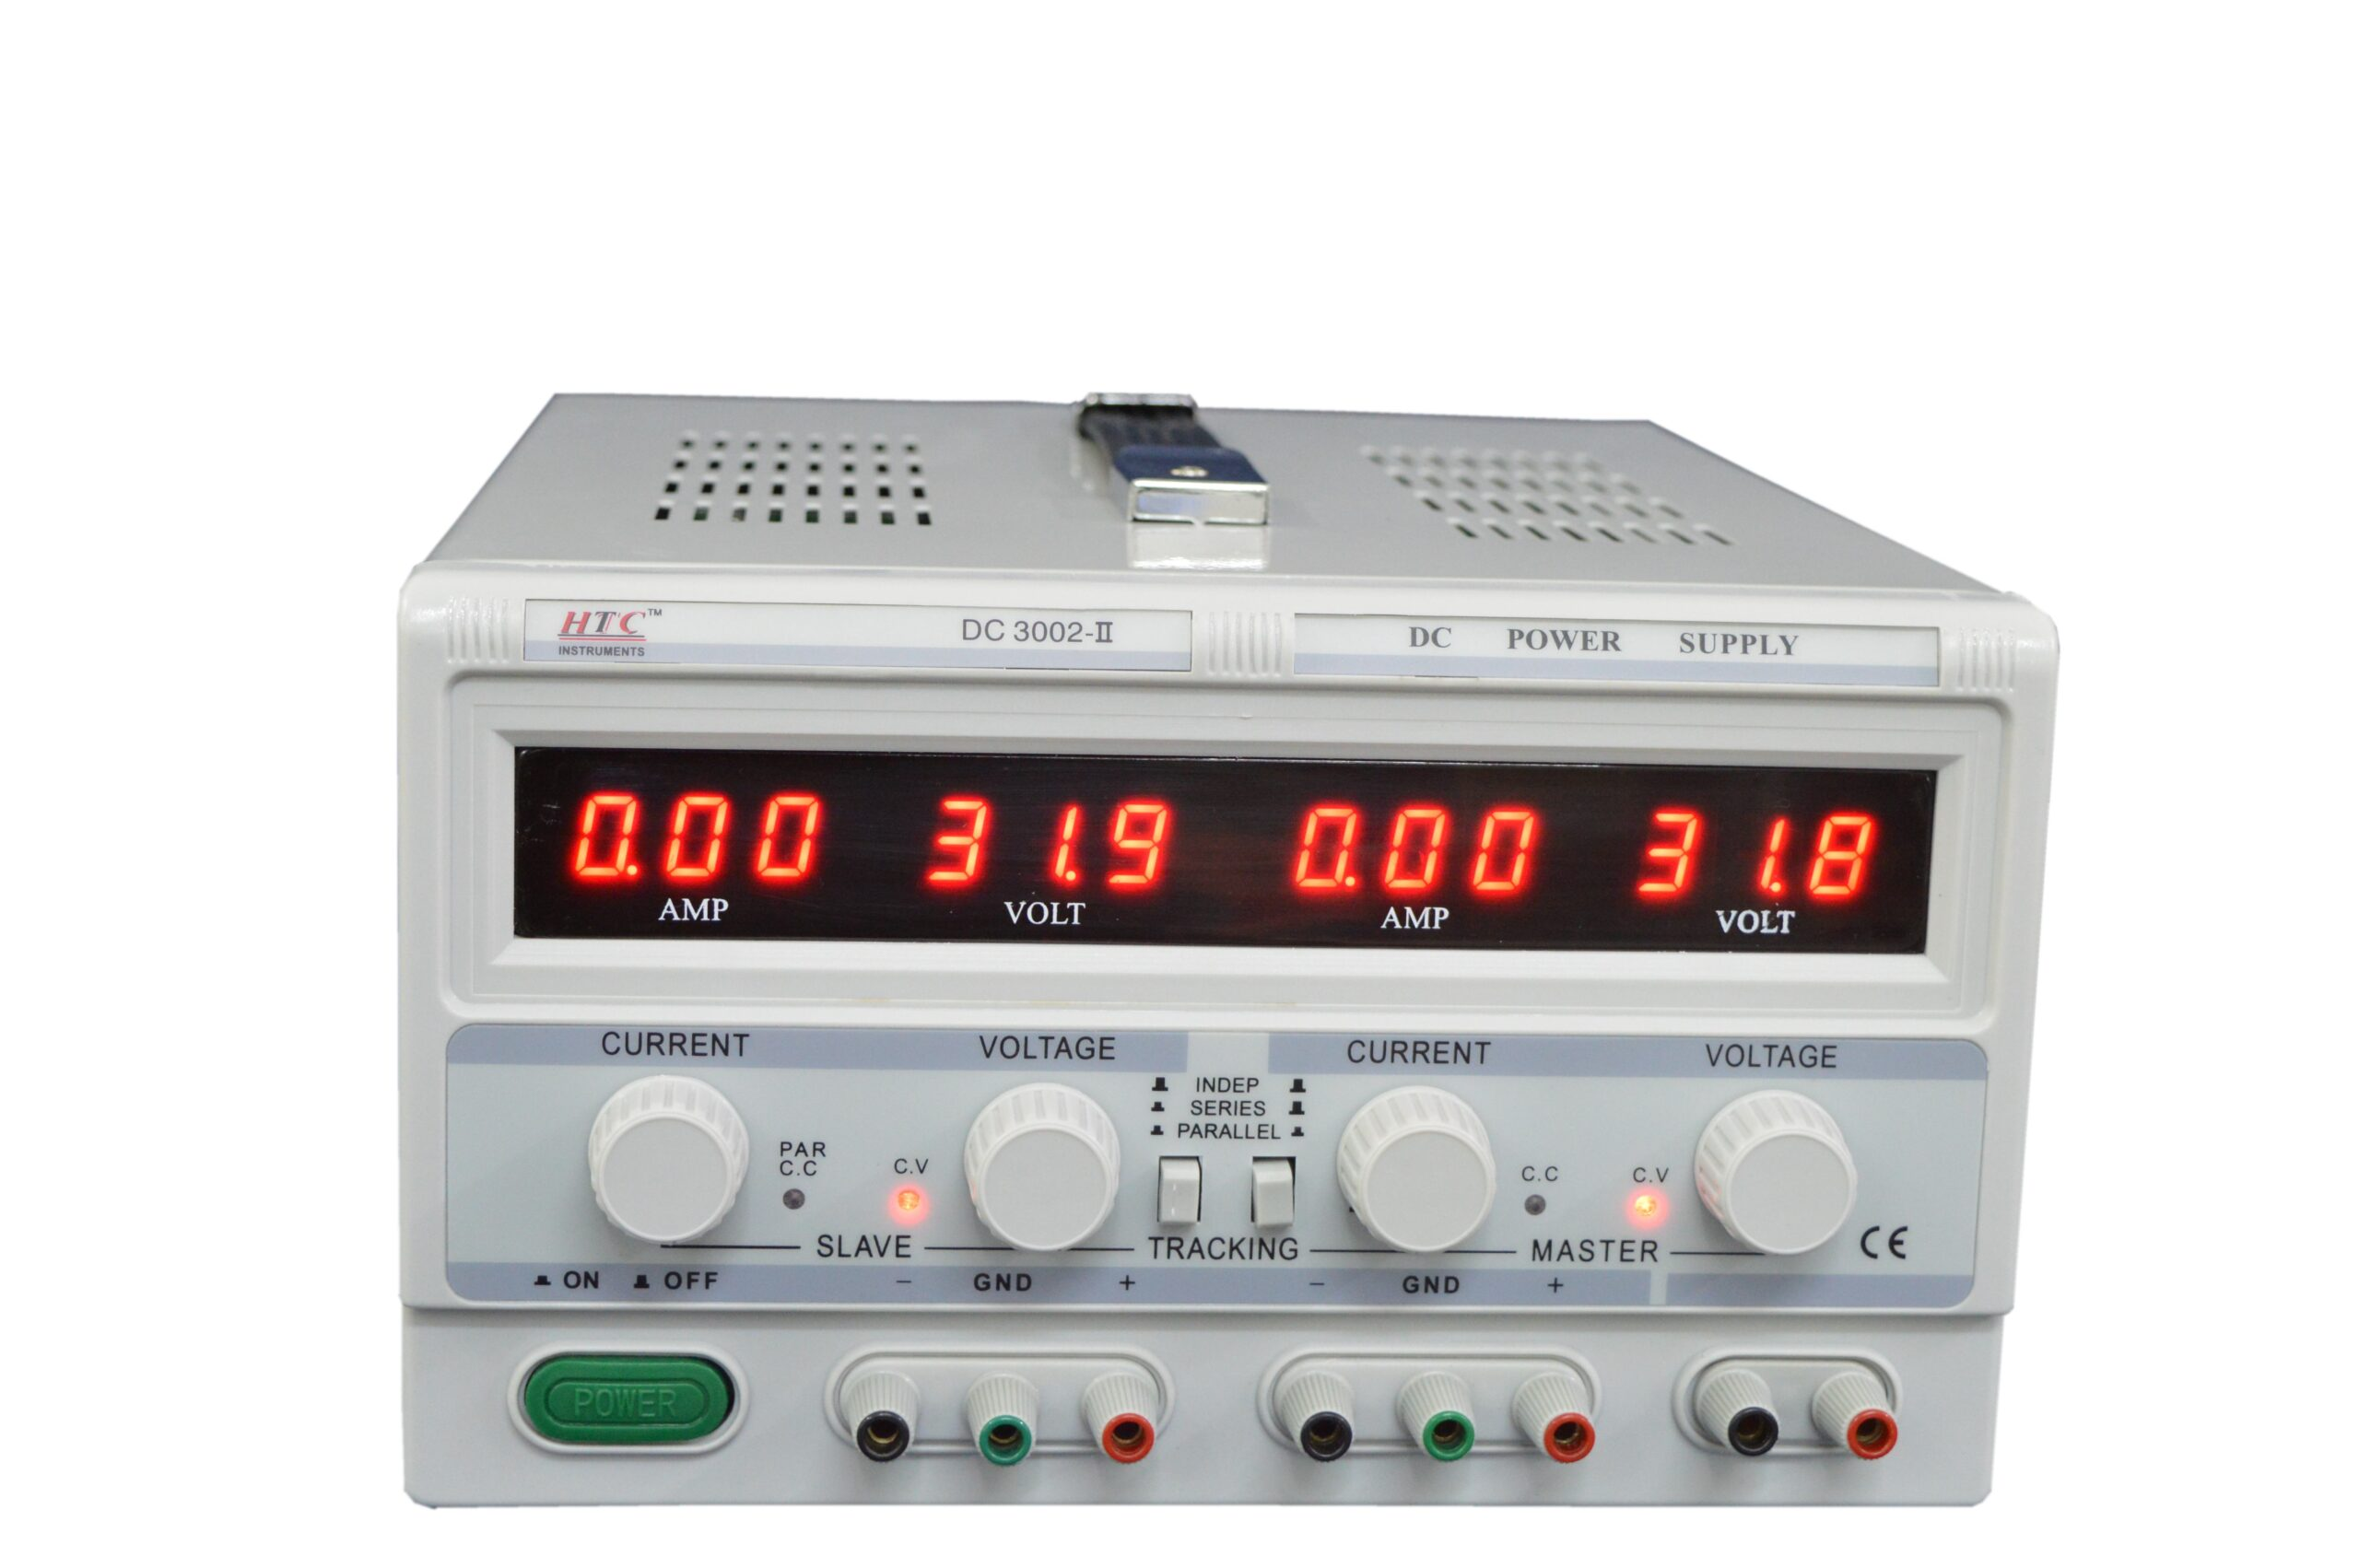
\includegraphics[width=0.5\textwidth]{./images/DC-PowerSupply.jpeg}
						\caption{DC power supply}
						\label{fig:DCPowerSupply}
					\end{figure}
				\item[Function generator] used to produce a signal
					\begin{figure}[h!]
						\centering
						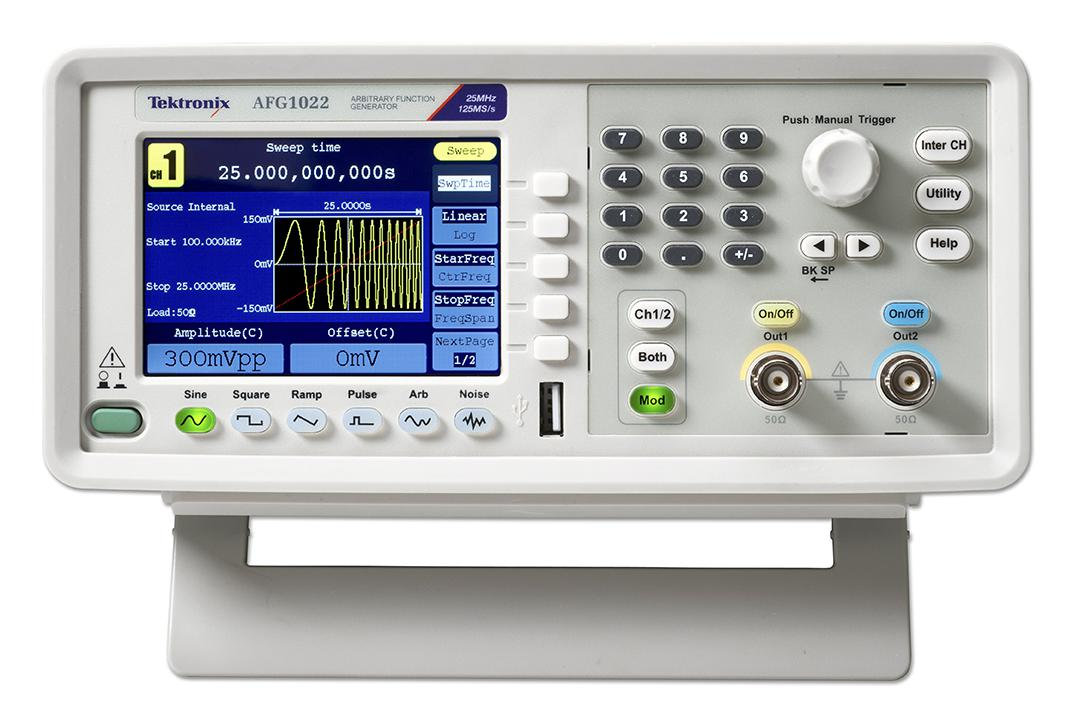
\includegraphics[width=0.5\textwidth]{./images/FunctionGenerator.jpeg}
						\caption{Function generator}
						\label{fig:FunctionGenerator}
					\end{figure}

				\item[Oscilloscope] used to show an signal
					\begin{figure}[h!]
						\centering
						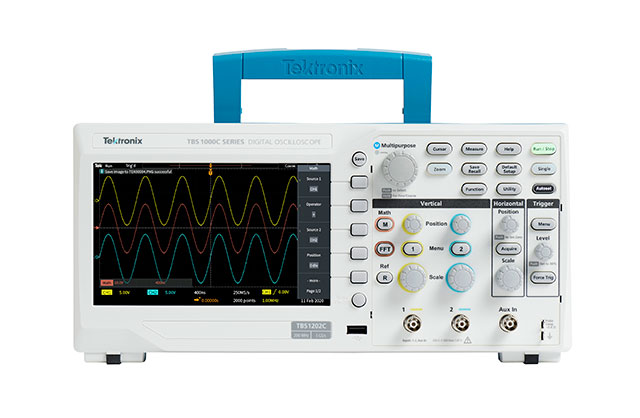
\includegraphics[width=0.5\textwidth]{./images/Oscilloscope.jpeg}
						\caption{Oscilloscope}
						\label{fig:Oscilloscope}
					\end{figure}

				\pagebreak

				\item[Probes] used to measure voltage
					\begin{figure}[h!]
						\centering
						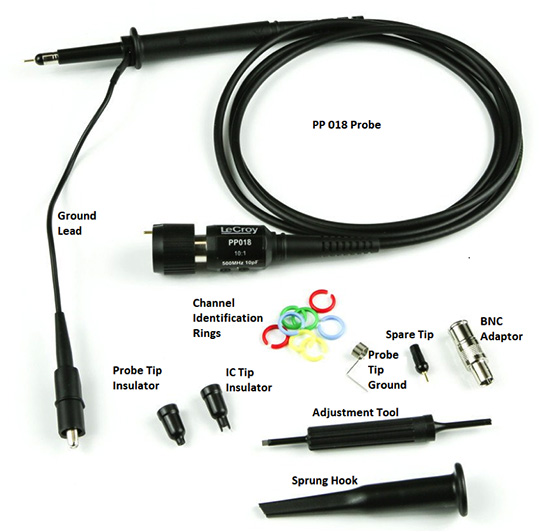
\includegraphics[width=\textwidth]{./images/Probe.jpeg}
						\caption{Probes}
						\label{fig:Probes}
					\end{figure}

				\pagebreak
				\item[Resistors] are used to control the current flow in circuits, they are mainly made of compost materials and their values which are given in Ohms can be found from color code (bands) on the resistor or by measuring the value of the resistance using Ohm-meter.
					Resistors and color code are shown in \figref{fig:ResistorColorCode}.
					\begin{figure}[h!]
						\centering
						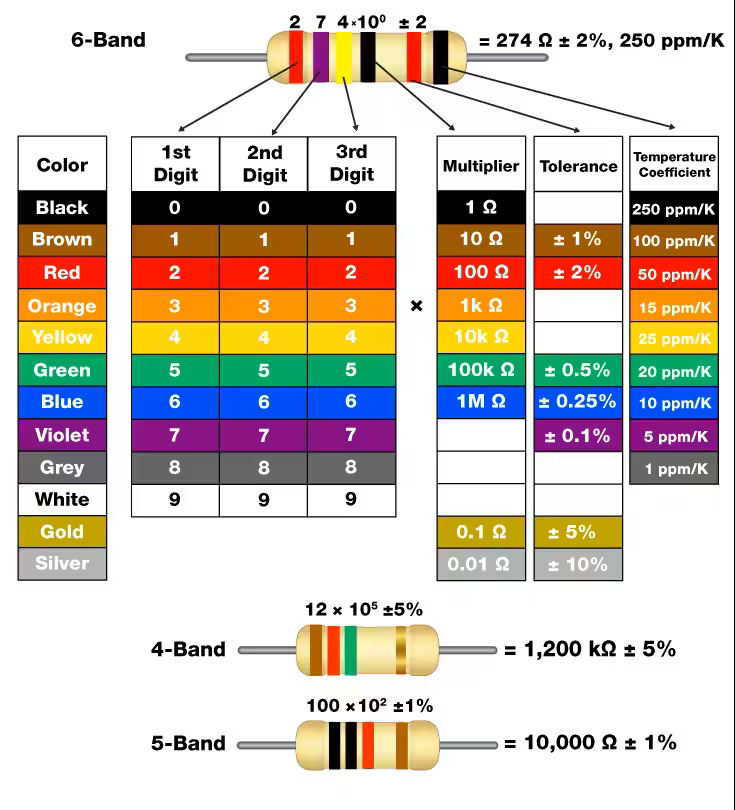
\includegraphics[width=\textwidth]{images/ResistorColorCode.png}
						\caption{Resistor color code table}
						\label{fig:ResistorColorCode}
					\end{figure}
			\end{description}
	
	\pagebreak
			\subsection{Procedure}
				To achive all of our goals we need to follow the following steps:
				\begin{enumerate}
					\item Switch in DC power supply, and fix it to 5 V, then measure the 5 V using the multi-meter
					\item When done switch off.
					\item Switch on the function generator, and fix it to produce sin wave with 100 Hz
					\item Measure and show the signal via a oscilloscope
					\item Switch them both off
					\item Pick up two unknown resistors, measure them using the multi–meter
					\item Connect them on bread board in series
					\item Connect them on the bread board in parallel
					\item Use more resistors and connect the circuit as shown in \figref{fig:Task8-Circuit}
				\end{enumerate}

				\subsubsection{Turning on the DC power supply}
					Here is a list of steps followed to turn on the DC power supply safely in the laboratory:
					\begin{enumerate}
						\item Connect the power supply to the power source
						\item Call an assistant to check the connections
						\item Turn on the power supply with the assistans approval
						\item Set the voltage to 5V
						\item Turn off the power supply
					\end{enumerate}

					Before measuring the voltage with the multi-meter, we decided to take some resisotrs and make a simple circuit of 3 resistors in a series connection and measure the voltage across the entire
					circuit and the voltage across each resistor.
				
				\pagebreak

				\subsubsection{Constructing the series circuit}
					We took 3 identical resistors, which were labaled to be $2200\Omega$ with some tolerance, and to be sure we measured them using a multimeter as can be seen at \figref{fig:MeasuringUnknownResistors}.
					\begin{figure}[h!]
						\centering
						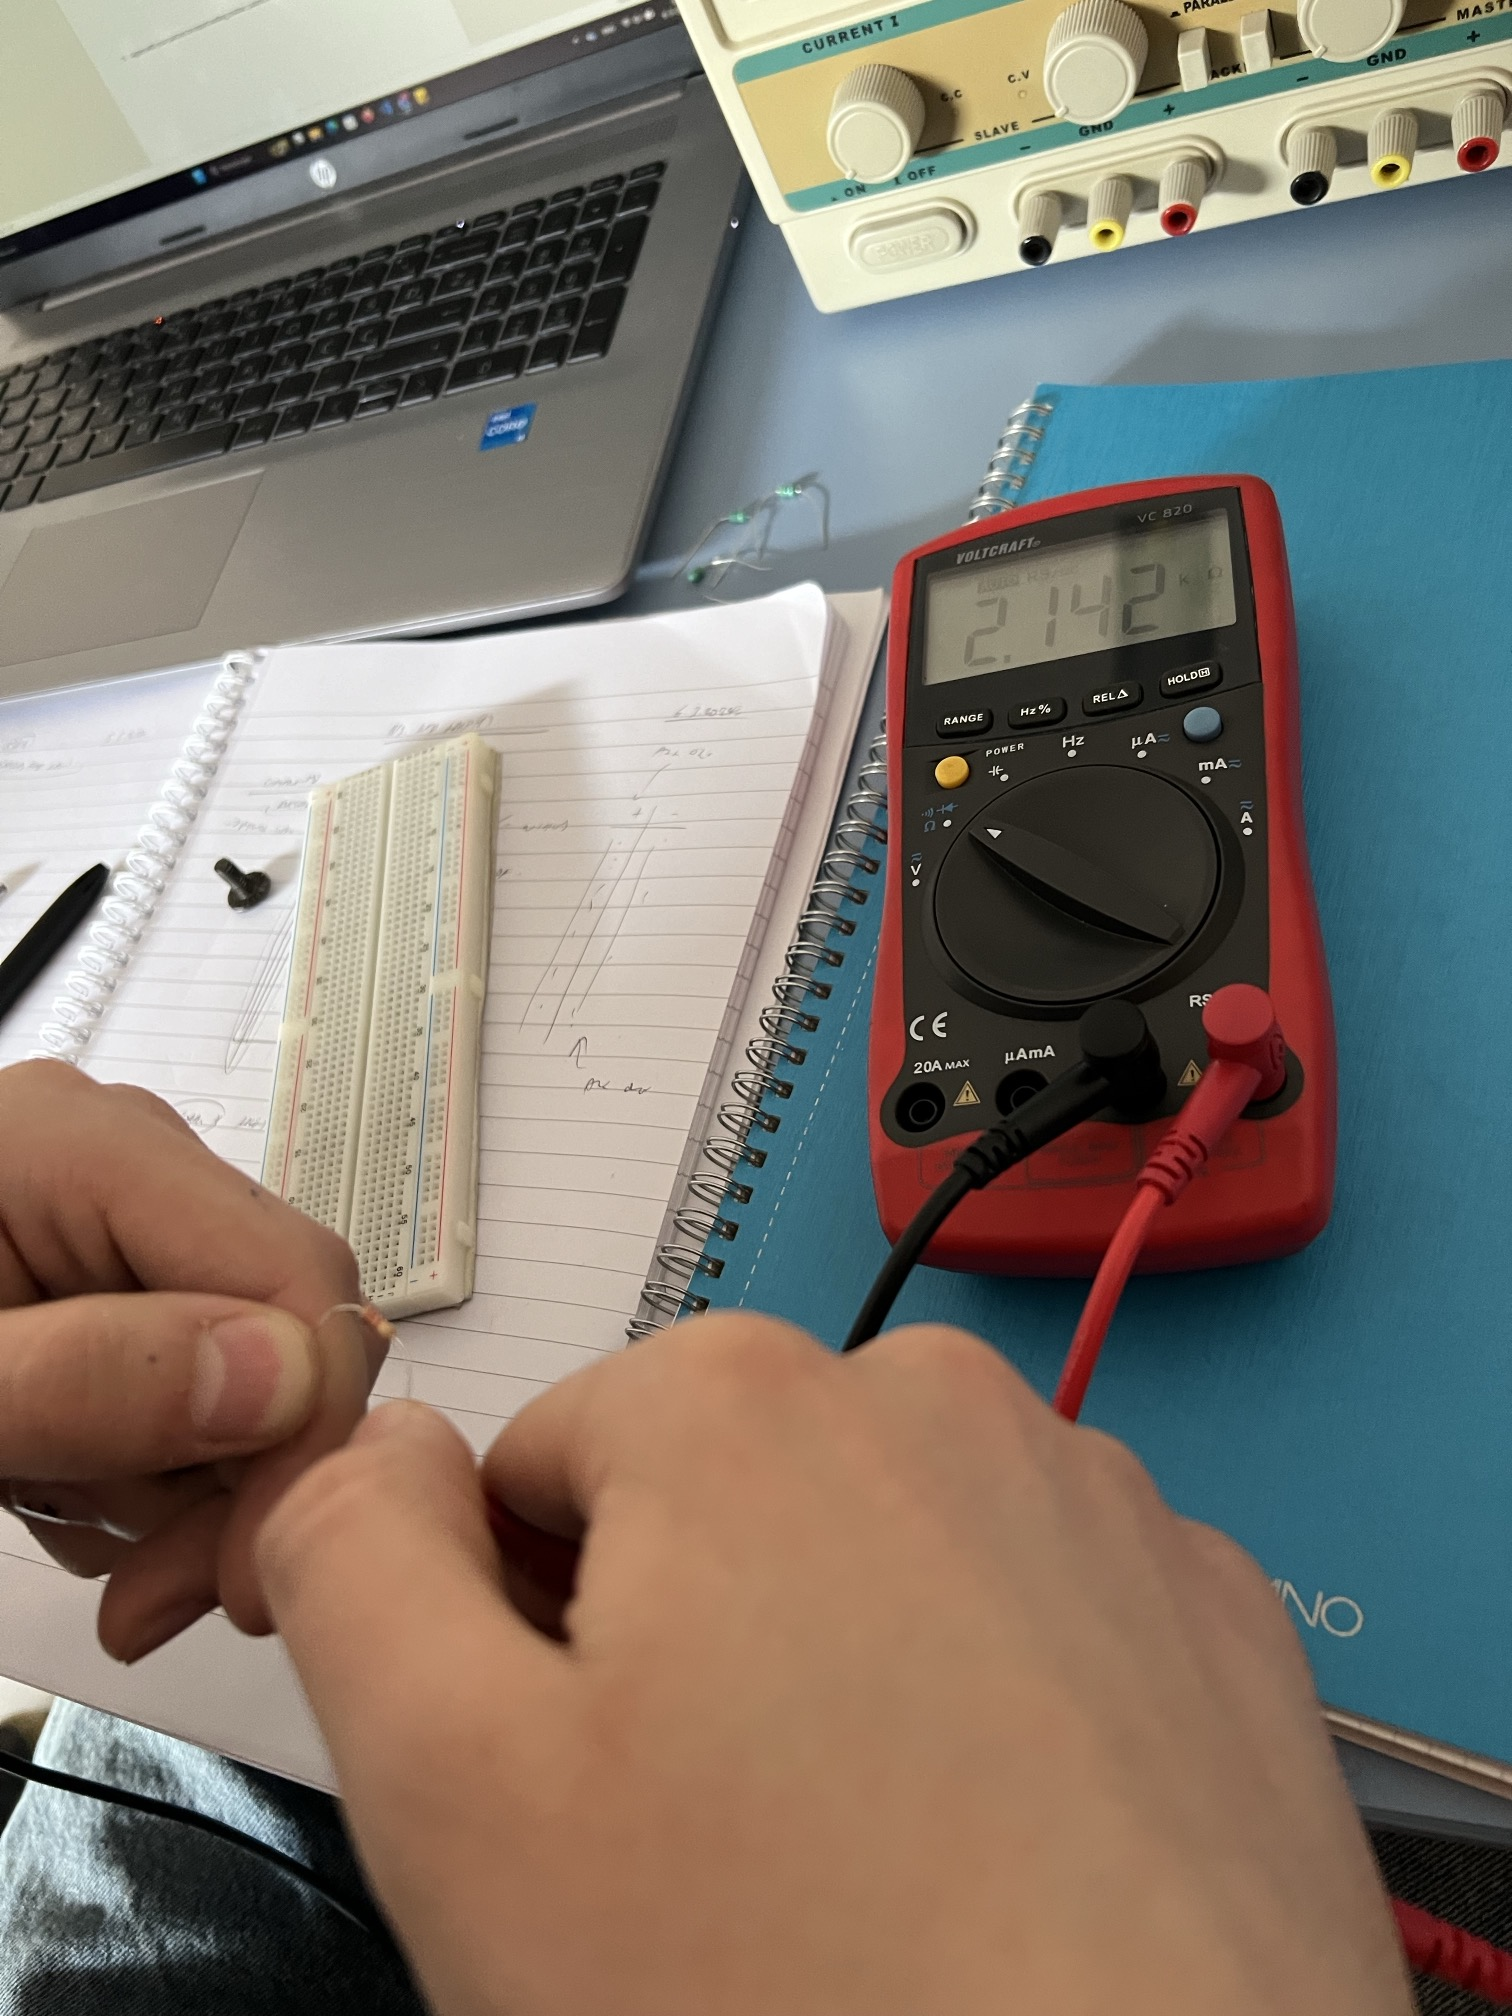
\includegraphics[width=0.35\textwidth]{./images/MeasuringUnknownResistors.jpeg}
						\caption{Measuring unknown resistors}
						\label{fig:MeasuringUnknownResistors}
					\end{figure}

					After setting up the multimeter to measure resistance, and after making sure the probes were connected properly to the multimeter,
					we measured the resistance of the first resistor to be $2.142\text{k}\Omega = 2142\Omega$. As we can see the tolerance of the resistor is $\pm 5\%$ (as shown by the golden ring).

					\vspace{5mm}

					Now we connected the resistors in series, and measured the voltage across the entire circuit and the voltage across each resistor.
					\begin{figure}[h]
						\centering
							\begin{subfigure}[h]{0.25\textwidth}
								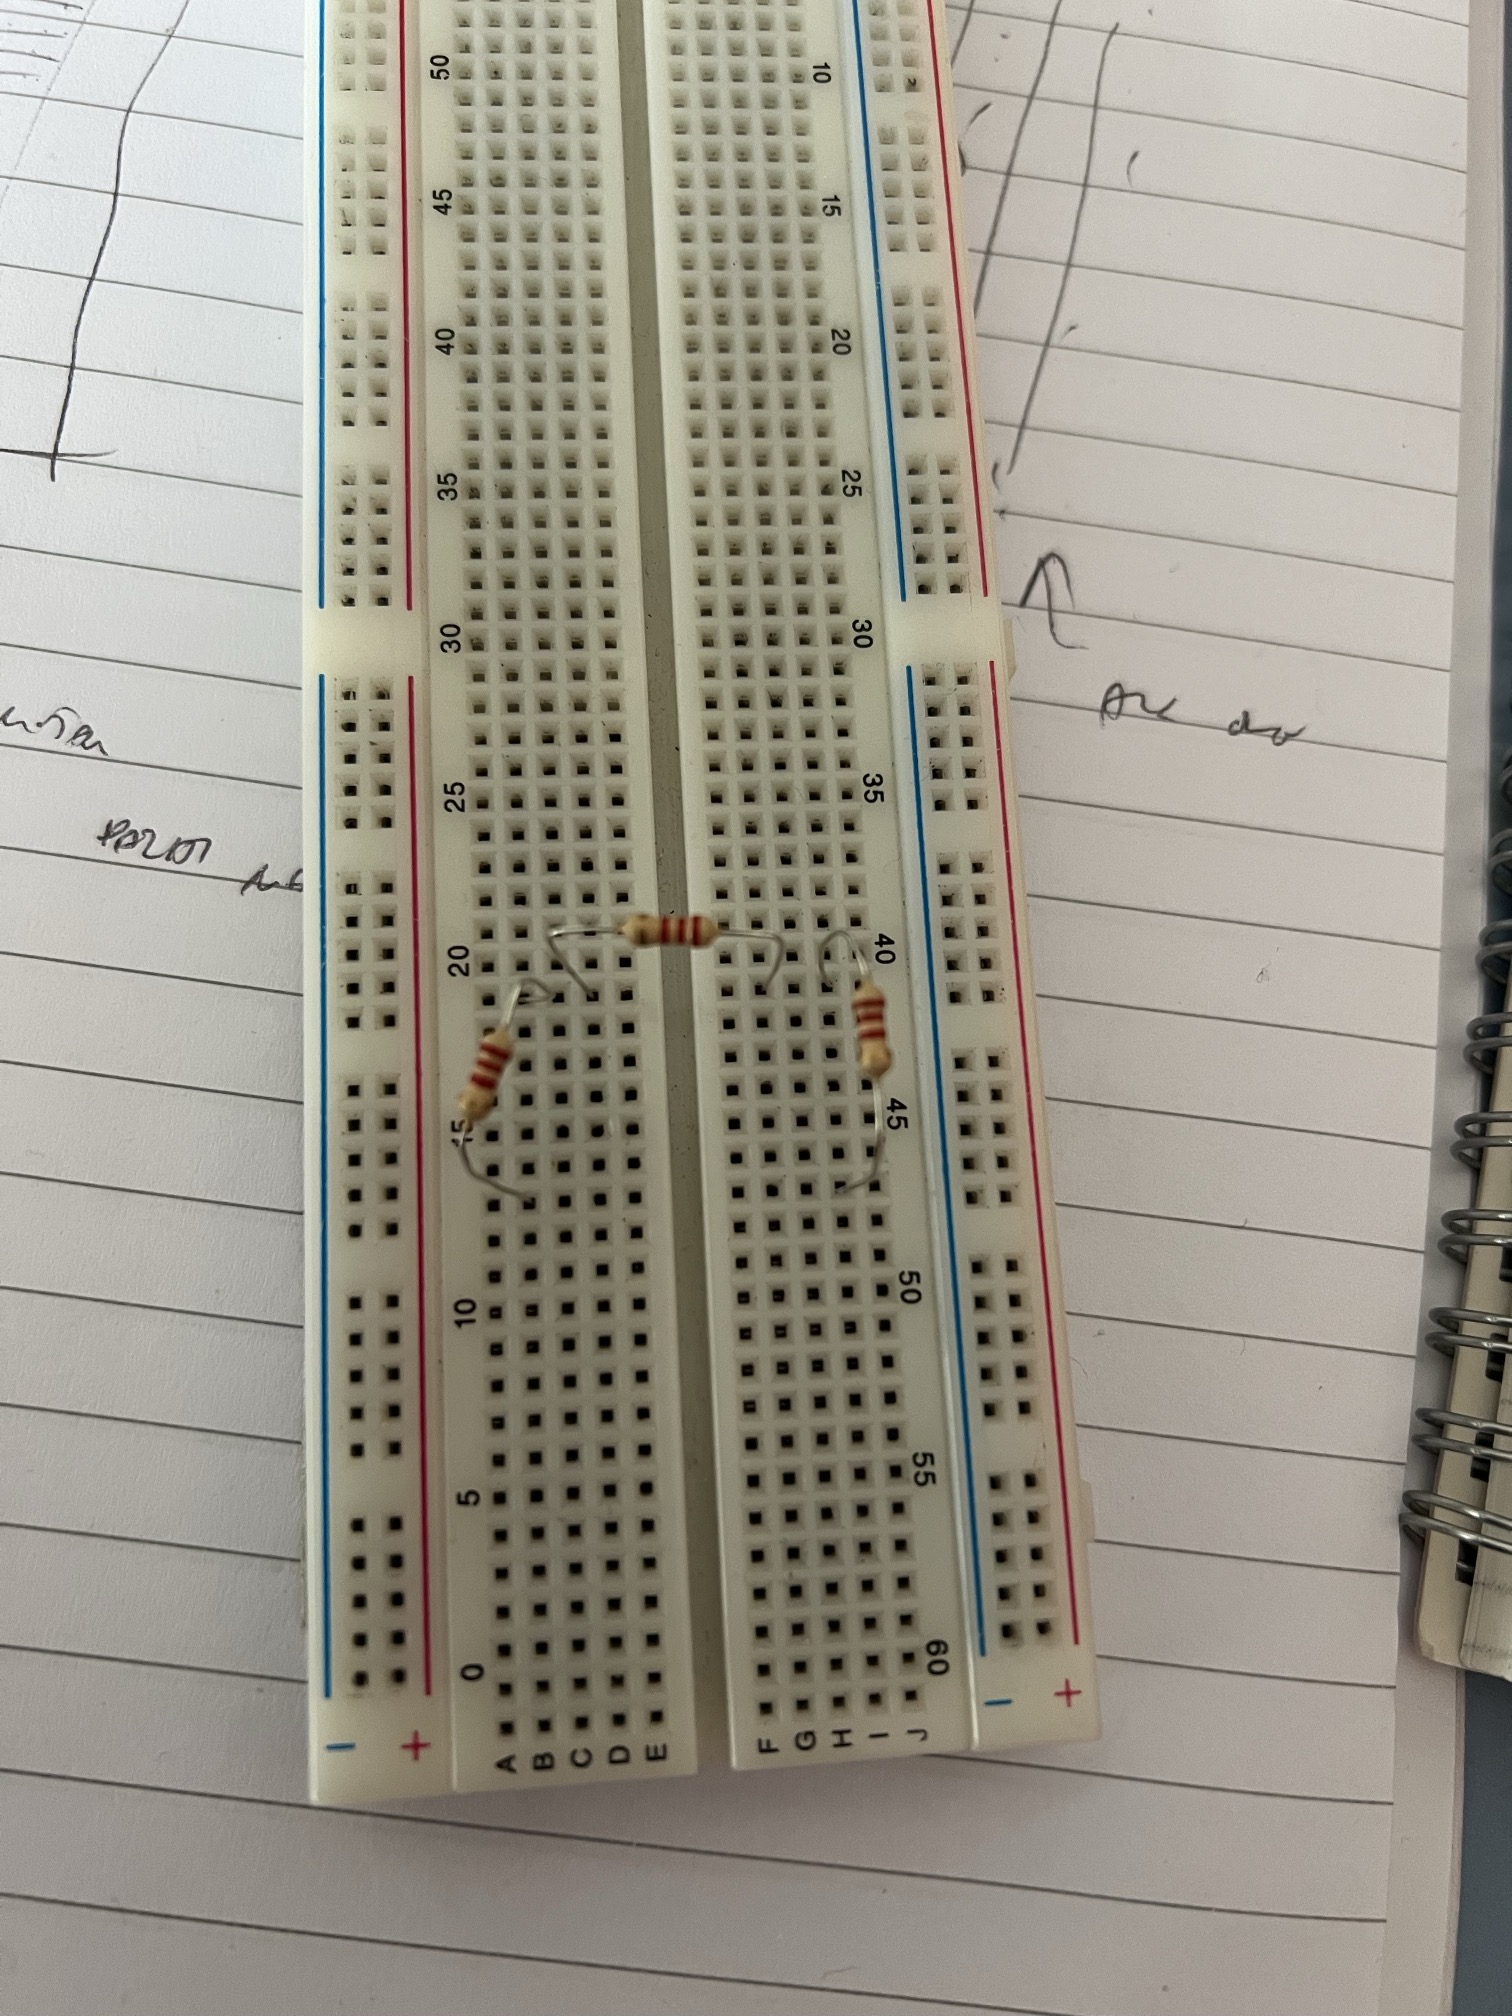
\includegraphics[width=\textwidth]{./images/SimpleCircuitInSeries.jpeg}
								\caption{Simple Circuit in series}
								\label{sub-fig:SimpleCircuitInSeries}
							\end{subfigure}
							\hspace{0.5cm} % This is the gap between the images
							\begin{subfigure}[h]{0.65\textwidth}
								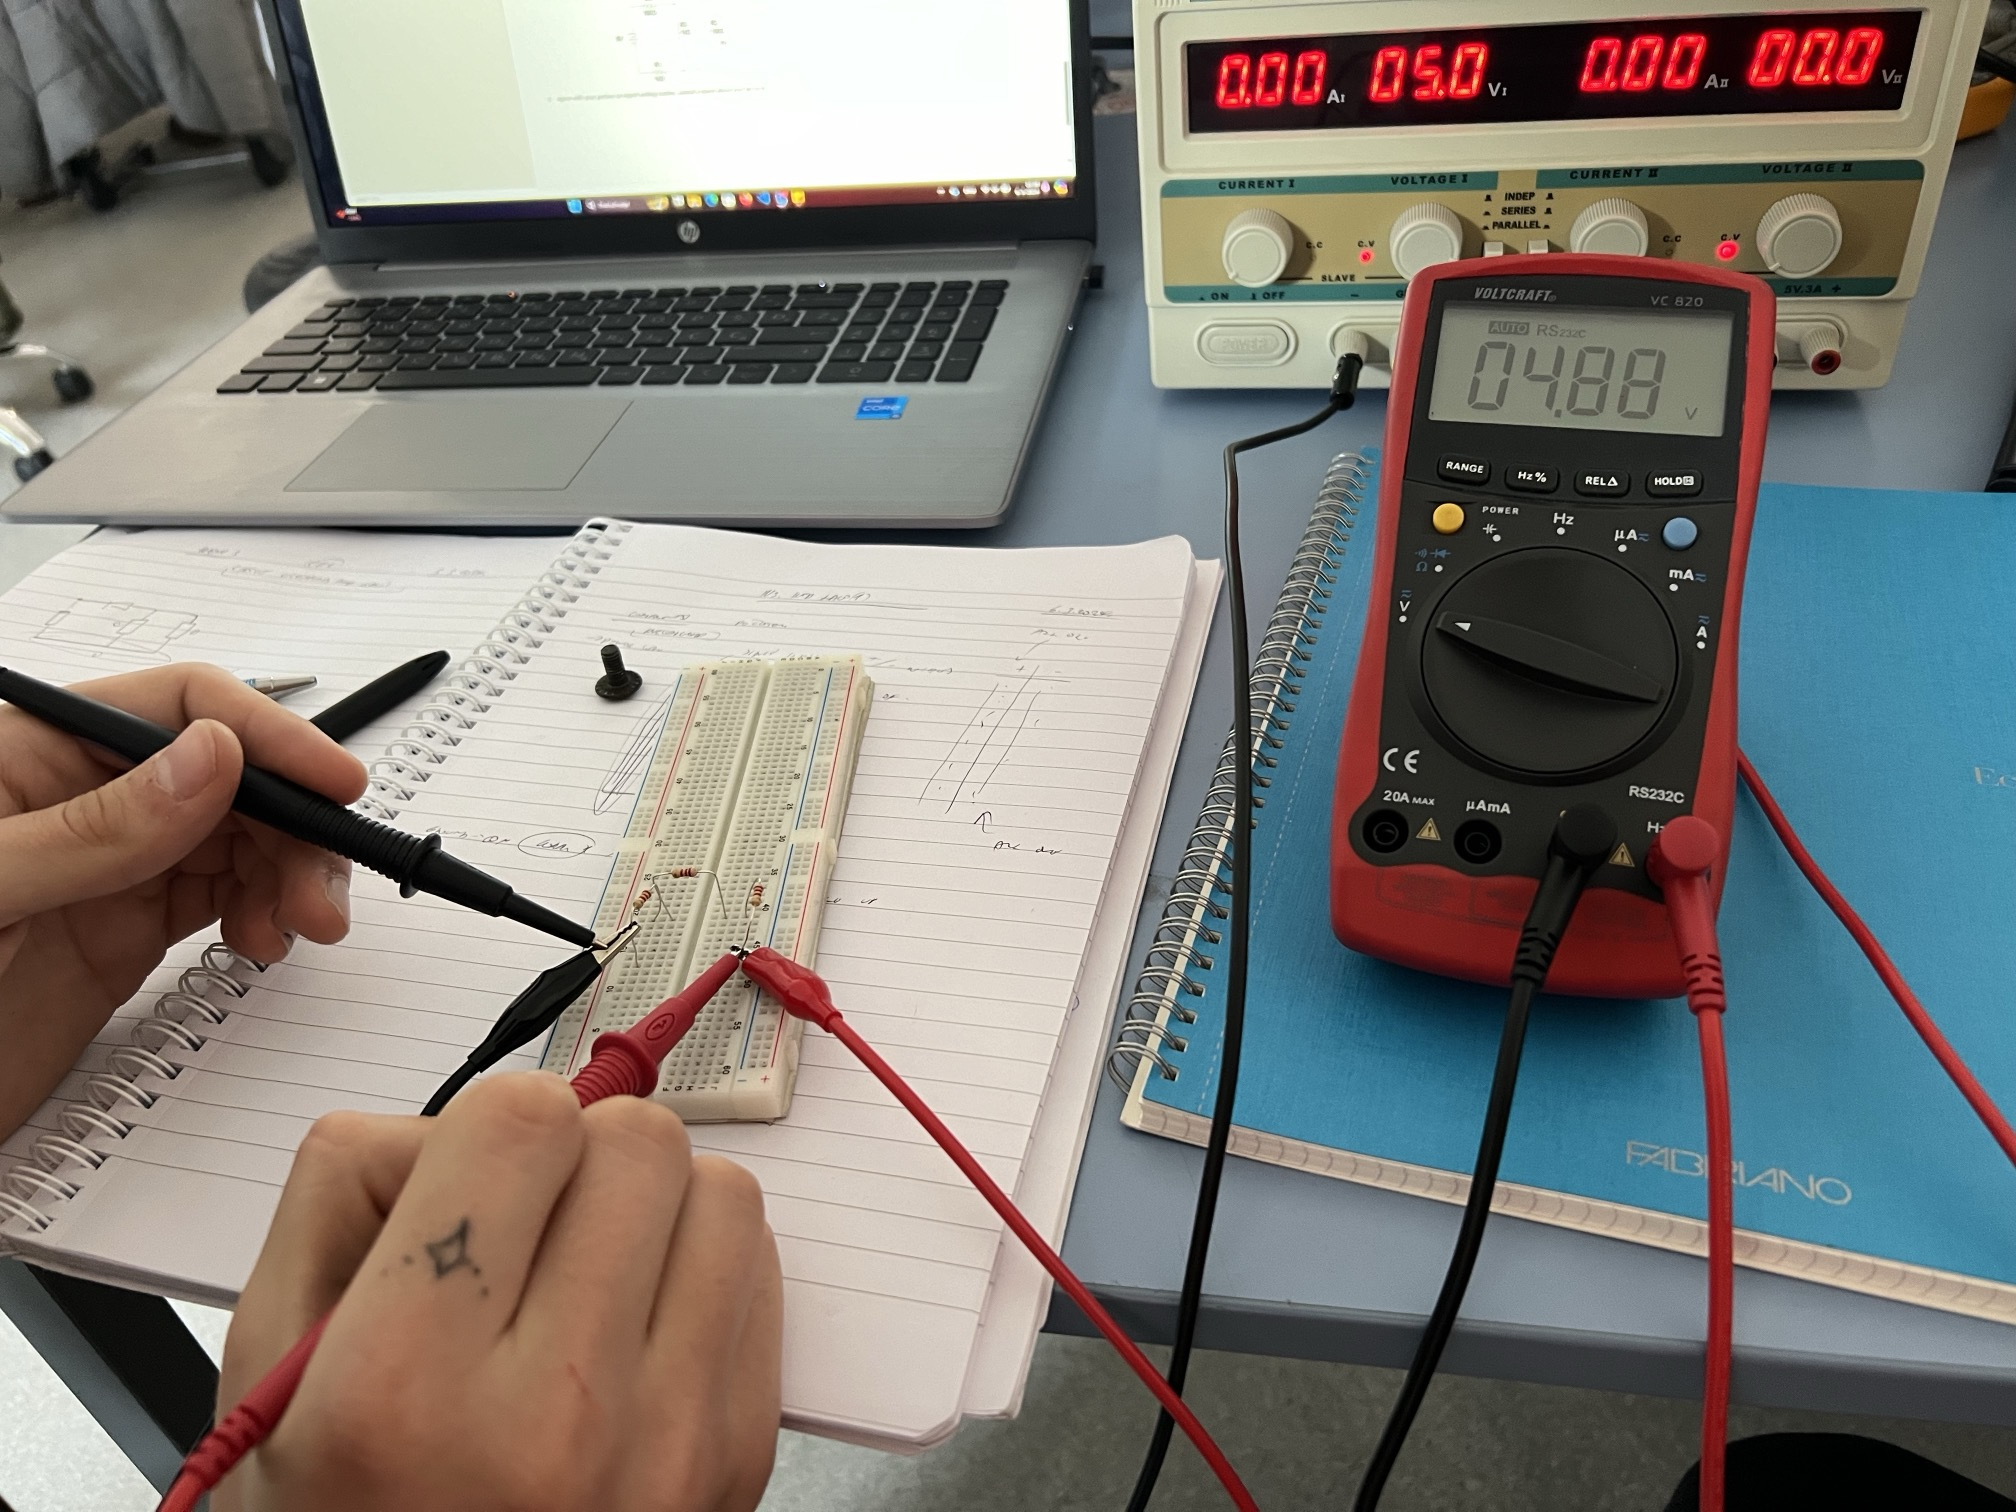
\includegraphics[width=\textwidth]{./images/MeasuringVoltageOfACircuit.jpeg}
								\caption{Multimeter measuring voltage over a simple circuit of 3 resistors in series}
								\label{sub-fig:MeasuringVoltageOfASimpleCircuit}
							\end{subfigure}

							\caption{Measuring voltage of a simple circuit}
							\label{fig:MeasuringVoltageOfACircuit}
					\end{figure}

					As we can see the voltage across the entire circuit is $4.8\text{V}$, and the voltage of the power supply is set to be $5.0\text{V}$. The reason for this difference, as stated by the
					lab assistatns, is that the power supply is not perfect and it has some internal resistance, which causes the voltage to drop when a load is connected to it, and the 
					probes used for the multimeter also have some resistance, which causes the voltage to drop when the multimeter is connected to the circuit. Another reason for the voltage drop is the
					inaccuracy of the multimeter, which is not perfect and has some tolerance same with the DC power supply. With this we conclude tasks with the DC power supply, parallel and series connection
					of resistors, and measuring the voltage across the entire circuit. One small note is that unfortunately we did not save our images of the parallel connection of resistors but you will be
					able to see a mixed connection when we get to the last task of the lab report.
				
				\subsubsection{Using and measuring the function generator}
					We turned on the function generator and set it to produce a sin wave with 100 Hz, and we connected the output of the function generator to the oscilloscope, and we measured the signal as shown in \figref{fig:MeasuringSignalWithOscilloscope}.
					\begin{figure}[h!]
						\centering
						\includegraphics[width=0.7\textwidth]{./images/MeasuringSignalWithOscilloscope.jpeg}
						\caption{Measuring signal with oscilloscope}
						\label{fig:MeasuringSignalWithOscilloscope}
					\end{figure}

					This part was very brief since we did not need to set up manually the volts/div and time/div, since the oscilloscope was already set up to measure the
					signal from the function generator. However in the future we were told that we would cover this in much more detail.

				
\end{document}
